\section{Theory and experimental setup}
ESSENTIALLY: STORM IS A METHOD FOR SMLM (j'avais eu un doute que c'était deux choses differentes mais non)

\subsection{Epifluorescence Microscopes}
A common architecture for fluorescence microscopes is that of an upright epifluorescence microscope, pictured in \autoref{fig:epifluorescence_microscope}.

\begin{figure}[htbp]  
    \centering
    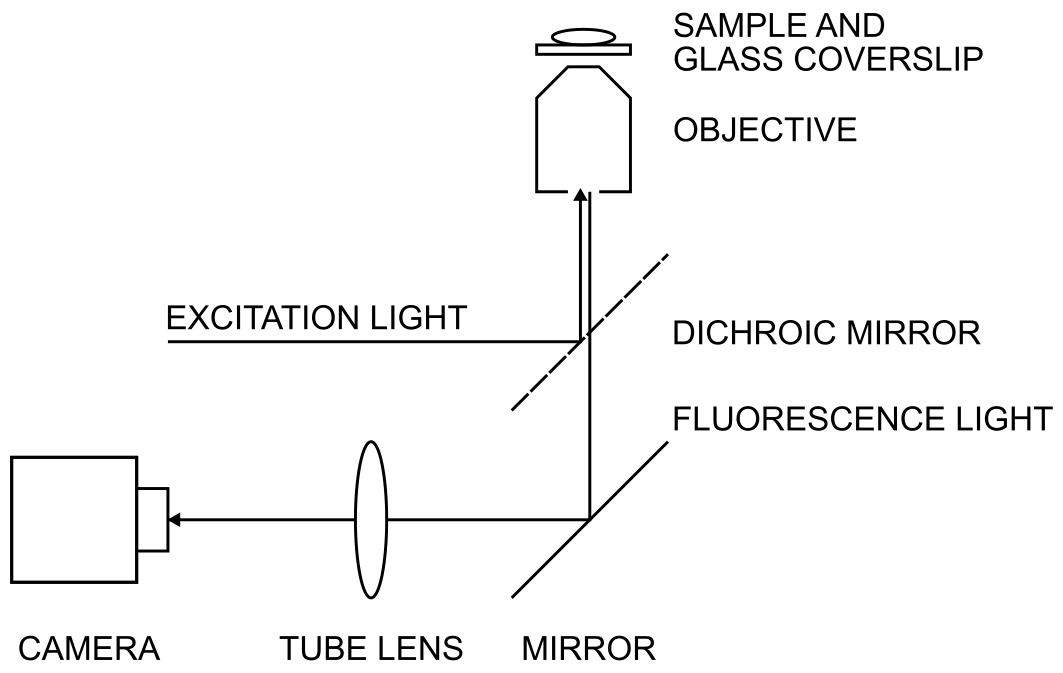
\includegraphics[width=8cm]{figures/epifluorescence-microscope.png}
    \caption{Epifluorescence microscope \cite{douglass_notice_2023} [can be put as wrapfig]}
    \label{fig:epifluorescence_microscope}
\end{figure}

Light emitted from a source such as a laser or a high-intensity LED enters the microscope and is reflected into the objective lens by a dichroic mirror, capable of reflecting some wavelengths of light and transmitting others (a passband filter)\cite{douglass_notice_2023}.
The excitation light is then focused by the objective lens onto the studied sample, where it excites the fluorescent molecules therein\footnote{lol} present.
The fluorescent light emitted by the molecules is collimated by the same objective lens and passes again through the dichroic mirror, which therefore acts as a beam splitter, separating the excitation and emission light paths\cite{sachl_introduction_2022}.
Finally, a second lens, known as tube lens, focuses the parallel rays coming from the objective lens and forms the image of the sample on the camera or eyepiece.
This setup using two lenses, called an infinity-corrected system, allows to add or replace optical elements (such as filters or additional beamsplitters) in the space between the two lenses (the infinity space) without disturbing/modifying the wavefront of the light and thus keeping the same focus and magnification.

This mode of observation, where the excitation light is delivered to the specimen by the same objective lens which is used for collecting the fluorescence, 
is known as epi-illumination.
\hl{The following is cut and copy, modifier}It solves the problem of the excitation light dominating the weaker fluorescence signal, as most of the excitation light propagates away from the objective after leaving  the sample.

THINGS WHICH CAN BE REMOVED IF SPACE IS NECESSARY:
Epi-illumination iluminates the whole samople at once, in order to BLABLA. 
Other illumination geometries include BLABLABLA.
Also people use reversed epifluorescence microscopes which are better for this and that.



\subsection{The Point Spread Function}
The PSF is a tool/way to characterise the performance of a microscope.
EXPLANATION OF PSF WITH FORMULAS


\subsection{Single Molecule Localization Microscopy}
How a single molecule is localised (CAN MAYBE GO IN PSF? IDK LA NOTICE SÉPARE LES DEUX)

(AUSSI ON POURRAIT METTRE PHOTOPHYSICS AVANT, PUIS EXPLIQUER TOUT D'UN COUP SMLM ET STORM (CÀD COMMENT ON LOCALISE UNE MOLECULE ET COMMENT ON SWITCH ON ET OFF POUR PRENDRE 10,000 PHOTOS ET RECONSTRUIRE UNE IMAGE))


\subsection{Fluorescence Photophysics}
The behaviour of Fluorophores, the energetic states (rapidly), Photoswitching (not Photoactivation because that's used in PALM, but we're doing STORM)

[the density of molecules being read out
    (that is, in an emissive state) at the same time must stay low
    enough for the distance between emitting molecules to be large
    compared to the diffraction limit, so that individual fluorophores
    can be spatially resolved] \hl{utile lorsqu'on explique STORM}.

\subsection{Experimental setup}
All results contained in this document were obtained using an Abbelight SAFe 180 Single Molecule Localization Microscope, an Oxxius ?? laser engine and a Hamamatsu ORCA-Fusion digital CMOS camera.
Three different laser wavelengths were used: \mbox{488 nm}, \mbox{561 nm} and \mbox{647 nm}.

To test the performance of the microscope, the localization precision of single fluorescente molecules was estimated.
Tetraspeck Microspheres, 0.1 $\mu$m diameter fluorescent beads.

Then STORM imaging of tubulin. Tubulin in COS7 cells labeled with AlexaFluor 647 fluorescent dye.

Then mitochondria, also using AlexaFluor 647 as fluorescent marker for the mitochondrial outer membrane in COS7 cells.
Data acquisition was conducted using the NEO Live Imaging software, while the STORM data was analysed with the NEO Analysis software.


\subsection{UTILE POUR ÉCRIRE:}
Selected quotes from \cite{furstenberg_single-molecule_2013}:
\begin{quote}
    Super-resolution methods that combine photoswitchable
    fluorophores with single-molecule imaging achieve their superior
    spatial resolution by temporally breaking down the total fluores-
    cence into pieces in which the signal level allows single emitters to
    be observed. To that end, the density of molecules being read out
    (that is, in an emissive state) at the same time must stay low
    enough for the distance between emitting molecules to be large
    compared to the diffraction limit, so that individual fluorophores
    can be spatially resolved. \cite{furstenberg_single-molecule_2013}
\end{quote}
\begin{quote}
    In essence, single-molecule localization microscopy relies on
    three basic points (Fig. 3): (i) the use of photoswitchable
    fluorescent probes, (ii) the repeated detection of many isolated
    emitters and the determination of their position (localization),
    and (iii) the generation of a super-resolution image from single-
    molecule localization data. In each imaging frame, only few
    molecules are allowed to reside in their fluorescent state
    (‘‘on’’ state), so that single emitters can be spatially resolved
    and localized despite a high labelling density. The majority of
    the labels are kept in their non-fluorescent state (‘‘off’’ state) in
    a stochastic way, most commonly dependent on the irradiation
    intensity or a chemical reagent. The contrast between the on
    and off states is crucial as the signal-to-background ratio will
    determine the precision of the localization. \cite{furstenberg_single-molecule_2013}
\end{quote}
\begin{quote}
    The simplest
    approach for estimating the lateral position (x, y) of an emitter
    is to calculate the intensity-weighted centroid of the detected
    intensity distribution. Another possibility is to fit a model
    function that resembles the point-spread function (PSF) of
    the microscope system to the detected intensity distribution
    of single emitters. Two-dimensional Gaussian normal distribu-
    tions or a radial Airy pattern are frequently chosen as model
    functions. The fitting can be performed either by least-squares
    minimization or by maximum likelihood estimation algo-
    rithms.71,73,74 A third method is the correlation of the data
    with a known intensity distribution of the microscope PSF. \cite{furstenberg_single-molecule_2013}
\end{quote}